
\subsection{Neural Networks} \label{sec:NN}
In den letzten Jahren gab es eine Vielzahl von Fortschritten durch Computersysteme, die häufig unter dem Begriff \ac{KI} zusammen gefasst werden. So konnte zum Beispiel AlphaGo einen der weltweit besten Spieler in dem Brettspiel Go schlagen und das System DeepFace ist in der Lage, menschliche Gesichter nahezu auf menschlichen Niveau erkennen zu können.\footcites[Vgl.][]{spiegelGoogleComputerAlphaGo2016}\footcite[Vgl.][]{taigman2014deepface}

Systeme die als \ac{KI} bezeichnet werden, sind häufig in der Lage, Aufgaben zu bewältigen, die bisher ausschließlich durch das menschliche Gehirn bearbeitet werden konnten. Neben den oben genannten Beispielen zählt hier auch das Erkennen von Bildern oder Sprache dazu. Damit Computer diese Aufgaben erledigen können, haben Wissenschaftler sich vom menschlichen bzw. biologischen Gehirn inspirieren lassen. Systeme, die auf dieser Grundlage basieren und einige der Vorgehensweisen des Gehirnen imitieren, werden als \ac{NN} bezeichnet.

\subsubsection{Aufbau}
Die grundlegenden Bausteine von \ac{NN} sind Perceptron und wurden 1958 von Rosenblatt beschrieben.\footcite[Vgl.][]{rosenblattPerceptronProbabilisticModel1958} Als Grundlage verwendete er hierbei unter anderem die Arbeit von McCulloch und Pitts.\footcite[Vgl.][]{mccullochLogicalCalculusIdeas1943}

\tikzset{%
  neuron missing/.style={
    draw=none, 
    scale=3,
    text height=0.333cm,
    execute at begin node=\color{black}$\vdots$
  },
}

\begin{figure}[t]
	\centering
	\begin{tikzpicture}[x=1.5cm, y=1.5cm,  >=stealth]
        \tikzstyle{unit}=[draw,shape=circle,minimum size=1.2cm]
        \tikzstyle{weight} =[draw, shape=rectangle, minimum size=.8cm]


        \node[unit](x1) at (0,3.5){$I_1$};
        \node[unit](xn) at (0,1.5){$I_{N}$};
        \node(dots) at (0,2.5){\vdots};
        \node[unit](bias) at (0,0){$b$};

        \node[weight](w1) at (2,3){$w_1$};
        \node[weight](wn) at (2,1.5){$w_n$};
        \node[weight](wb) at (2,0.5){$w_b$};

        \node[unit](wSum) at (4,1.5){$\sum$};

        \draw[->] (bias) -- (wb);
        \draw[->] (x1) -- (w1);
        \draw[->] (xn) -- (wn);
        \draw[->] (wb) -- (wSum);
        \draw[->] (w1) -- (wSum);
        \draw[->] (wn) -- (wSum);

        \draw [->] (wSum) -- ++(1,0)
        node [above, midway] {};
        
        \end{tikzpicture}
	\caption[]{Darstellung eines Perceptron}
    \label{fig:perceptron}
    Quelle: Eigene Darstellung, 2020
\end{figure}

Ein Perceptron kann zwischen $1$ und $n$ Eingangssignalen sowie einen negativen Bias Term\footnote{Einige Defintionen schreiben nicht vor, dass der Bias negativ sein muss. Stattdessen wird dieser im weiteren Vorgehen subtrahiert statt summiert zu werden} $b$ erhalten und hieraus ein Ausgangssignal - auch Aktivierung genannt - erzeugen. Für das Ausgangssignal werden alle Eingangssignale jeweils mit einem eigenen - als Gewicht bezeichneten - Faktor multipliziert (siehe Abbildung \ref{fig:perceptron}). Die Ergebnisse werden anschließend zusammen mit dem Bias summiert. Ist die Summe kleiner oder gleich $0$, ist der Ausgangswert ebenfalls $0$, ansonsten beträgt der Ausgangswert $1$. Der Bias stellt also den Schwellwert dar, den die gewichtete Summe überschreiten muss, damit das Ausgangssignal $1$ lautet. 

Es ist möglich, ein Perceptron um eine Aktivierungsfunktion zu ergänzen, sodass das Ausgabesignal reelle Werte annehmen kann. Diese Erweiterung des Perceptron wird als Neuron bezeichnet. Weit verbreitet ist die Verwendung der Sigmoid Funktion (siehe Gleichung \ref{eq:sigmoid}). Bei der Anwendung einer Aktivierungsfunktion, häufig mit $\sigma$ dargestellt, wird die gewichtete Summe $z$ in die gewählte Funktion gegeben und das Ergebnis stellt das Ausgangssignal des Neuron dar (siehe Gleichung \ref{eq:outputNeuron}).

\begin{equation} \label{eq:sigmoid}
    \sigma (z) =  \frac{1}{1+e^{-z}}
\end{equation}

\begin{equation} \label{eq:outputNeuron}
    a = \sigma (\sum_{i}{x_i w_i + b})
\end{equation}

Neben der Sigmoid Funktion werden in modernen \ac{NN} häufig die ReLu Funktion (Gleichung \ref{eq:ReLU}) oder die tanh Funktion (Gleichung \ref{eq:tanh}) verwendet. Alle drei werden in Abbildung \ref{fig:activationfunctions} gegenüber gestellt. Es ist zu erkennen, dass sowohl bei der Sigmoid Funktion, als auch bei der ReLU Funktion die untere Grenze des Wertebereichs bei $0$ liegt. Bei der tanh Funktion, liegt diese bei $-1$. Außerdem haben nur die Sigmoid- und tanh Funktion eine obere Grenze - beide 1 - definiert. ReLU kann jeden Wert größer gleich $0$ annehmen. Verwendet man eine Aktivierungsfunktion, stellt der Bias kein Schwellwert mehr dar. Er ist als einziger Term in der Berechnung des Wertes der in die Aktivierungsfunktion gegeben wird von den Eingangswerten unabhängig und sorgt somit um eine konstante Verschiebung.

\begin{equation} \label{eq:ReLU}
    ReLU(z) = max(0,z)
\end{equation}

\begin{equation} \label{eq:tanh}
    \tanh(z) = \frac{\sinh(z)}{\cosh(z)} = \frac {e^z - e^{-z}} {e^z + e^{-z}}
  = \frac{e^{2z} - 1} {e^{2z} + 1}
\end{equation}

\begin{figure}[t]
    \centering
    \caption[]{Darstellung der Sigmoid-, ReLU- und tanh Funktion}
	\label{fig:activationfunctions}
    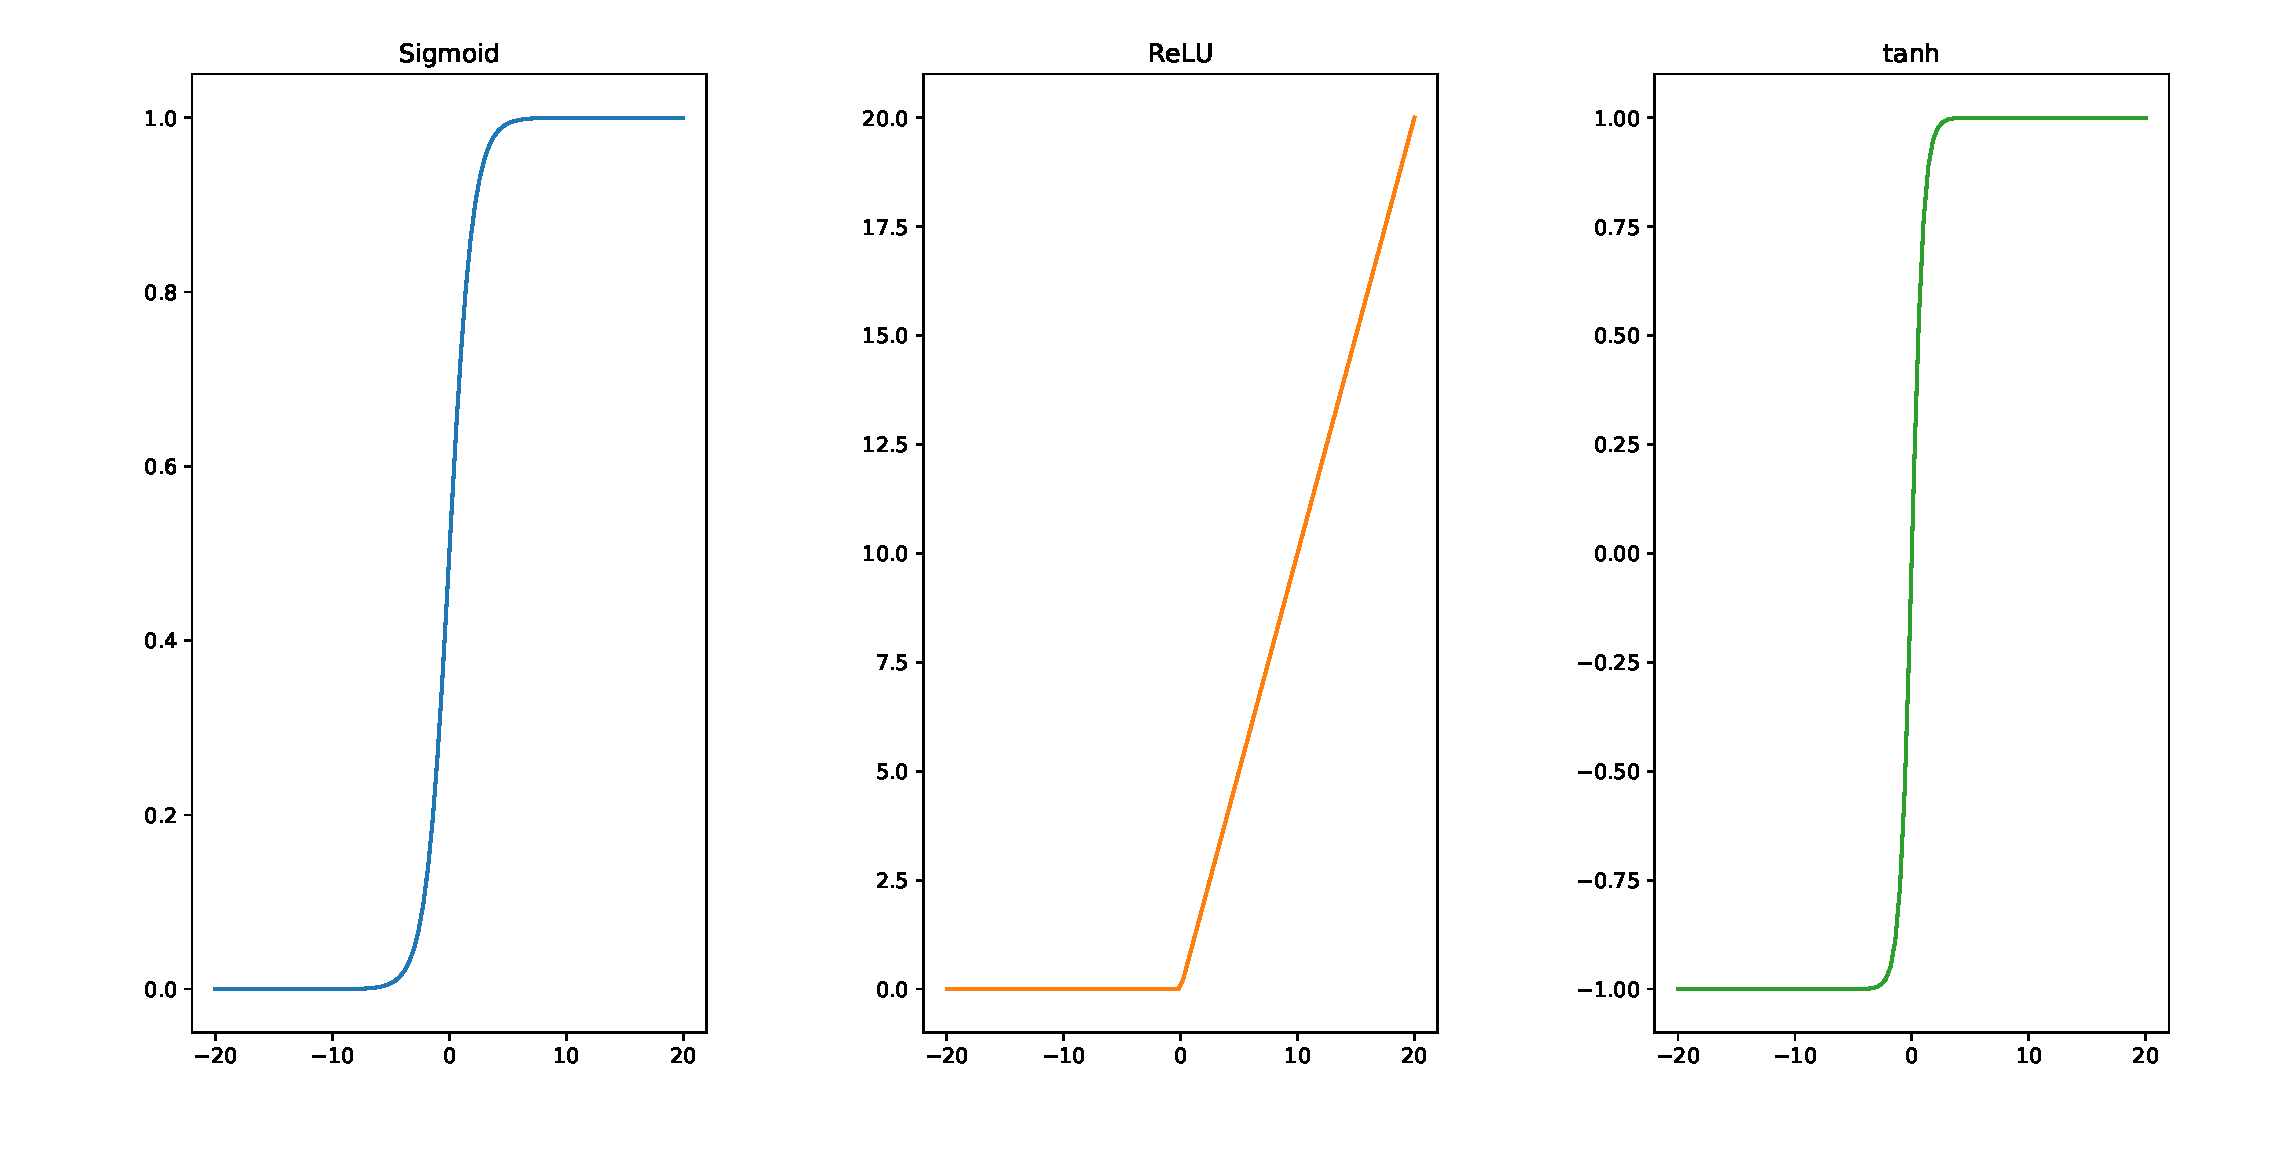
\includegraphics[width=1\textwidth]{activationfunctions.eps}
    Quelle: Eigene Darstellung, 2020
\end{figure}

Ein \ac{NN} besteht aus mehreren, verschalteten Neuronen. Diese werden in Layern angeordnet, welche typischerweise mit $1$ bis $N$ durchnummeriert werden. Layer 1 wird außerdem als Input Layer bezeichnet, da dieser die einzelnen Eingangswerte in das \ac{NN} darstellt. Layer N wiederum wird als Output Layer bezeichnet, da er das Ergebnis des \ac{NN} ausgibt. Alle Layer dazwischen (1 < $l$ < N) werden als Hidden Layer bezeichnet, da von außen weder direkt auf die Eingangssignale der Neuronen in diesen Layern Einfluss genommen werden kann, noch die Ausgabesignale dieser direkt ersichtlich sind. Jeder Layer kann dabei eine unterschiedliche Anzahl von Neuronen enthalten. Typischerweise sind die Neuronen in einem Layer mit allen Neuronen des vorherigen Layers verbunden, ist dies der Fall, wird der Layer auch \textit{Dense Layer} bezeichnet. Eine allgemeine Darstellung eines \ac{NN} mit drei Layern ist in Abbildung \ref{fig:multilayer-perceptron} dargestellt.
\tikzset{%
  every neuron/.style={
    circle,
    draw,
    minimum size=1.2cm
  },
  neuron missing/.style={
    draw=none, 
    scale=3,
    text height=0.333cm,
    execute at begin node=\color{black}$\vdots$
  },
}

\begin{figure}[t]
	\centering
	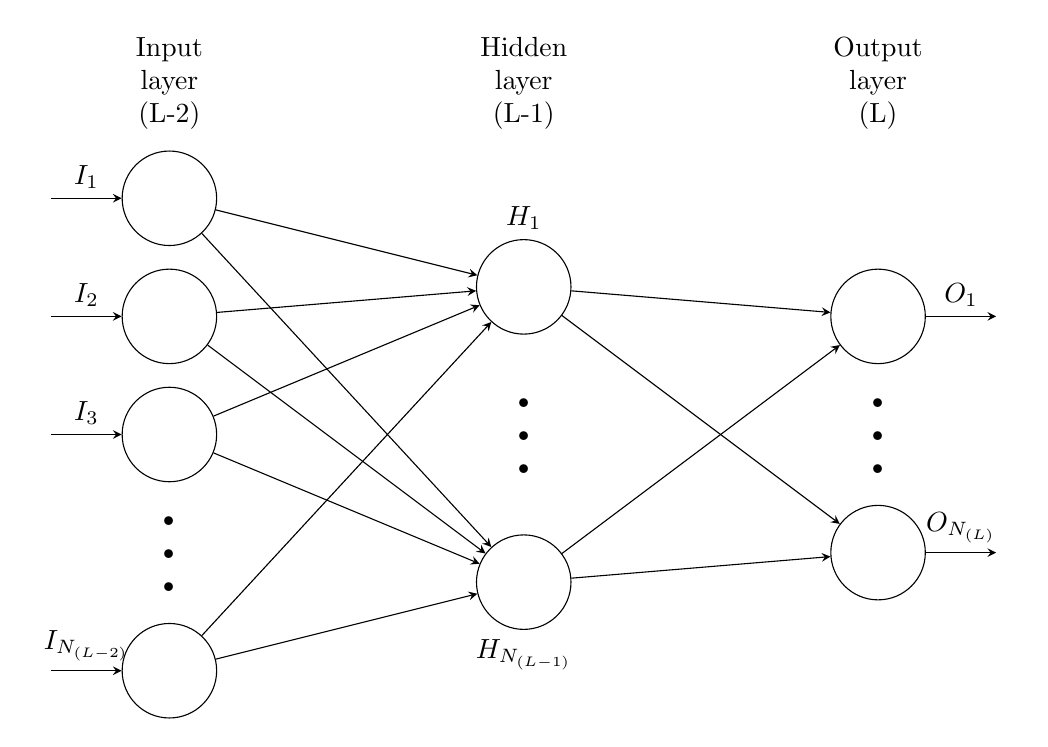
\begin{tikzpicture}[x=1.5cm, y=1.5cm,  >=stealth]

        \foreach \m/\l [count=\y] in {1,2,3,missing,4}
          \node [every neuron/.try, neuron \m/.try] (input-\m) at (0,2.5-\y) {};
        
        
        \foreach \m [count=\y] in {1,missing,2}
          \node [every neuron/.try, neuron \m/.try ] (hidden-\m) at (3,2-\y*1.25) {};
        
        \foreach \m [count=\y] in {1,missing,2}
          \node [every neuron/.try, neuron \m/.try ] (output-\m) at (6,1.5-\y) {};
        
        \foreach \l [count=\i] in {1,2,3}
          \draw [<-] (input-\i) -- ++(-1,0)
            node [above, midway] {$I_\l$};
        \draw [<-] (input-4) -- ++(-1,0)
            node [above, midway] at (input-4) {$I_{N_{(L-2)}}$};
        
        \node [above] at (hidden-1.north) {$H_1$};
        \node [below] at (hidden-2.south) {$H_{N_{(L-1)}}$};
        
        
        \draw [->] (output-1) -- ++(1,0)
        node [above, midway] {$O_1$};
        \draw [->] (output-2) -- ++(1,0)
        node [above, midway] {$O_{N_{(L)}}$};
        
        \foreach \i in {1,...,4}
          \foreach \j in {1,...,2}
            \draw [->] (input-\i) -- (hidden-\j);
        
        \foreach \i in {1,...,2}
          \foreach \j in {1,...,2}
            \draw [->] (hidden-\i) -- (output-\j);
        
        %\foreach \l [count=\x from 0] in {Input, Hidden, Ouput}
        \node [align=center, above] at (0*2,2) {Input \\ layer \\ (L-2)};
        \node [align=center, above] at (1.5*2,2) {Hidden \\ layer \\ (L-1)};
        \node [align=center, above] at (3*2,2) {Output \\ layer \\ (L)};
        
        \end{tikzpicture}
	\caption[]{Allgemein Darstellung eines Neural Network mit 3 Layern}
    \label{fig:multilayer-perceptron}
    Quelle: Eigene Darstellung, 2020
\end{figure}



\subsubsection{Gradient Descent}
Im Rahmen des Lernprozesses eines \ac{NN} werden die Gewichte und Bias der einzelnen Perceptron regelmäßig aktualisiert. Dabei liegt das Ziel darin, durch die Optimierung dieser Faktoren den Fehler des \ac{NN} bei der Vorhersage zu minimieren.

Um diesen Fehler bestimmen zu können, wird eine Verlustfunktion angewendet. Ein einfaches Beispiel einer Verlustfunktion basiert auf der mittleren quadratischen Abweichung.

\begin{equation} \label{eq:mse}
    C(w,b) = \frac{1}{2} \sum (y-\hat{y})^2
\end{equation}

In Gleichung \ref{eq:mse} werden die Gewichte mit \textit{w} und die Bias mit \textit{b} bezeichnet. Zusätzlich werden die wahren Klassen durch \textit{y} und die Ausgabe des \ac{NN} durch \textit{\^{y}} dargestellt. \todo{Prüfen ob variablen konsistent verwendet werden}


Um den Fehler des \ac{NN} zu minimieren, muss der globale Tiefpunkt der Verlustfunktion bestimmt werden. Bei Funktionen mit einer Vielzahl von Parametern, ist es zu komplex, diese Aufgabe analytisch zu lösen. \textit{\ac{GD}} stellt einen iterativen Prozess dar, sich dem nächsten Minimum zu nähern. Bildlich kann dieser Vorgang mit einem Wanderer, der vom Gipfel eines Berges absteigen möchte, verglichen werden. Geht dieser von seinem aktuellen Standpunkt ein paar Schritte in die entgegengesetzte Richtung der steilsten Stelle am Berg und wiederholt diesen Vorgang immer wieder, wandert er immer weiter ins Tal. Betrachtet man Abbildung \ref{fig:quadLoss}, würde der Wanderer in einem der braunen Quadrate beginnen und sich Schritt für Schritt tiefer bis zum blauen Bereich vorarbeiten. 

Mathematisch gesehen kann dies als eine Funktion \textit{L(v)} gesehen werden, wobei \textit{v} eine beliebige Anzahl von Parametern darstellt. Für eine bessere Übersichtlichkeit, wird im folgendem mit zwei Parametern, \textit{v\textsubscript{1}} und \textit{v\textsubscript{2}} gerechnet.

\begin{figure}[t]
    \centering
    \caption[]{Beispiel quadratische Verlustfunktion mit den Parametern v\textsubscript{1} und v\textsubscript{2}}
	\label{fig:quadLoss}
    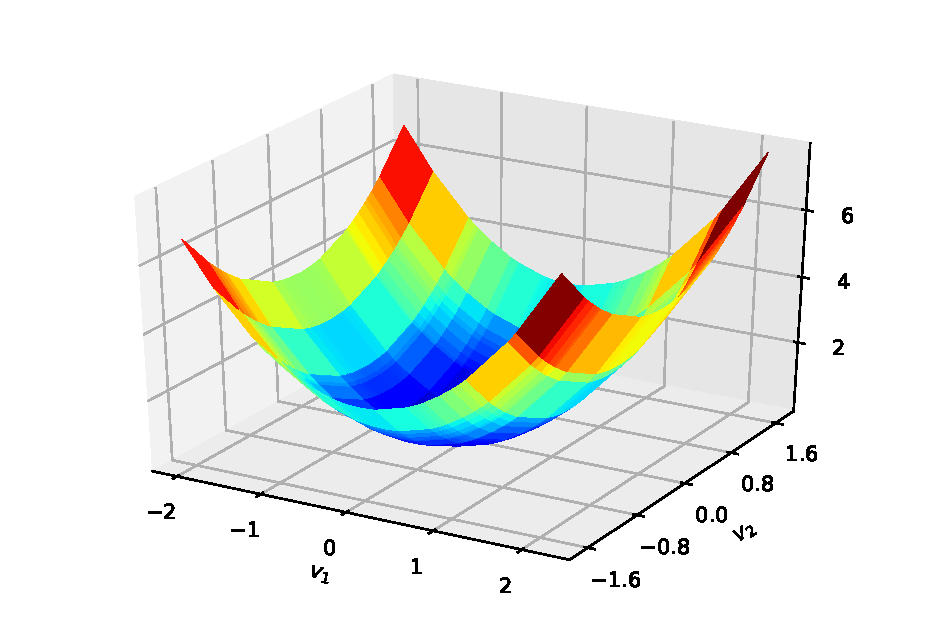
\includegraphics[width=1\textwidth]{quadratic_loss_function.eps}
    Quelle: Eigene Darstellung, 2020
\end{figure}

\begin{equation} \label{eq:deltaL}
    \Delta C \approx \frac{\partial C}{\partial_{v1}} \Delta v_{1} + \frac{\partial C}{\partial_{v2}} \Delta v_{2}
\end{equation}

In Gleichung \ref{eq:deltaL} wird die Funktion $\Delta$L als Summe der partiellen Ableitungen von \textit{v\textsubscript{1}} und \textit{v\textsubscript{2}} definiert. Die hierdurch erhaltenen Gradienten zeigen in die Richtung der größten Änderungen von \textit{v\textsubscript{1}} beziehungsweise \textit{v\textsubscript{2}} .

Fasst man die Parameter \textit{v\textsubscript{1}} und \textit{v\textsubscript{2}} und die partiellen Ableitungen jeweils in einem Vektor zusammen (Gleichung \ref{eq:vector1} und \ref{eq:vector2}), kann Gleichung \ref{eq:deltaL} zu Gleichung \ref{eq:vereinfachung1} umgeformt werden. $\Delta$v kann hierbei als der Vektor der Veränderung der Parameter gesehen werden.

\begin{equation} \label{eq:vector1} 
    \Delta v \equiv \binom{\Delta v_{1}}{ \Delta v_{2}}
\end{equation}

\begin{equation} \label{eq:vector2}
    \nabla C \equiv (\frac{\     C}{\partial_{v1}},  \frac{\partial C}{\partial_{v1}})^{T}
\end{equation}

\begin{equation} \label{eq:vereinfachung1}
    \Delta C \approx \nabla C \cdot \Delta v
\end{equation}

Um den Gesamtverlust zu reduzieren, muss der Vektor $\Delta$v in jedem Durchgang aktualisiert werden. Durch den Gradienten ist die Richtung der größten Änderung vom aktuellen Punkt der Funktion aus bekannt. Da der Gesamtverlust minimiert werden soll, muss in die entgegengesetzte Richtung des Gradienten gegangen werden. Dessen Wert wird also negiert. Außerdem muss eine positive Schrittweite bestimmt werden, die skaliert wie Weit in die Gegenrichtung des Gradienten gegangen wird. Diese wird als \textit{Learning Rate} und häufig mit $\alpha$ bezeichnet. Gleichung \ref{eq:learningRate} zeigt, wie die Veränderung der Parameter, $\Delta$v, mittels $\alpha$ skaliert und das Ergebnis negiert wird.

\begin{equation} \label{eq:learningRate}
    \Delta v = -\alpha \nabla C
\end{equation}      

Wird Gleichung \ref{eq:learningRate} in Gleichung \ref{eq:vereinfachung1} eingesetzt und umgeformt, erhält man Gleichung \ref{eq:finalGradDes}. Da  $\nabla C^2$ und $\alpha$ jeweils positiv sind, ist sichergestellt, dass die vorgenommene Veränderung negativ ist. Dies bedeutet, dass der Verlust mit jedem Durchgang verringert wird. Das \ac{NN} lernt also und seine Ausgaben weichen weniger von den wahren Werten ab. Anzumerken ist hierbei noch, dass das Minimum bei einer zu groß gewählten \textit{Learning Rate} überschritten werden kann. Dies würde dazu führen, dass man den Tiefpunkt überschreitet und wieder ein Stück hoch geht. Außerdem kann das erreichte Minimum ein lokales und nicht globales Minimum sein. Dies ist abhängig vom Startpunkt, da der negierte Gradient immer zum nächstgelegenen Minimum führt.

\begin{equation} \label{eq:finalGradDes}
    \Delta C \approx -\alpha \nabla C \cdot  \nabla C =  -\alpha \nabla C^2
\end{equation}

Ersetzt man \textit{v\textsubscript{1}} und \textit{v\textsubscript{2}} durch \textit{w} und \textit{b}, ist die Berechnung der neuen Werte für die Gewichte \textit{w\textsubscript{j}} und Bias \textit{b\textsubscript{j}} wie in den Gleichungen dargestellt \ref{eq:updateW} und \ref{eq:updateB} definiert.
\begin{equation} \label{eq:updateW}
    w_{j} \rightarrow w_{j}^{'} = w_{j} - \alpha \frac{\partial C}{\partial w_{j}}
\end{equation}

\begin{equation} \label{eq:updateB}
    b_{j} \rightarrow b_{j}^{'} = b_{j} - \alpha \frac{\partial C}{\partial b_{j}}
\end{equation}

\textit{\ac{GD}} betrachtet alle Beispiele im Trainingsdatensatz, bevor die Gewichte und Bias das erste Mal angepasst werden. Da dies  besonders bei großen Trainingsdatensätzen sehr zeit- und rechenintensiv ist, wird bei diesen Datensätzen häufig \ac{SGD}\footcite[Vgl. ][S. 400 ff.]{robbinsStochasticApproximationMethod1951}  angewendet. Bei \ac{SGD} werden die Anpassungen bereits nach einem oder einer Gruppe von Beispielen aus dem Datensatz durchgeführt. Dies hat zwar den Nachteil, dass die Optimierung der Verlustfunktion schlechter sein kann als bei \ac{GD}, allerdings konvergiert \ac{SGD} meistens schneller.

\subsubsection{Backpropagation}

Wie im letzten Abschnitt beschrieben, müssen für die Anwendung von \ac{GD}  $\frac{\partial C}{ \partial w}$ und  $\frac{\partial C}{ \partial b}$ berechnet werden. Rumelhart et al. haben für eine schnelle und effiziente Berechnung dieser im Jahre 1986 den Backpropagation Algorithmus vorgeschlagen.\footcite[Vgl. ][S. 533 ff.]{rumelhart1986learning} Dieser stellt eine Erweiterung der Delta-Regel auf \ac{NN} mit mehr als zwei Schichten dar.\todo[]{Quelle einfügen} Die Grundidee besteht darin, den Fehler des \ac{NN} auf die einzelnen Gewichte und Bias innerhalb des \ac{NN} zurückzuführen, so dass diese angepasst werden können. 
Formuliert man die Grundidee zum Beispiel für die Gewichte um, stellt sich die Frage, inwiefern sich der Fehler des \ac{NN} ändert, wenn das Gewicht $w_{jk}$ angepasst wird (siehe Gleichung \ref{eq:defDeltaEdef}).

\begin{equation} \label{eq:defDeltaEdef}
    \frac{\partial C}{ \partial w_{jk}}
\end{equation}

\begin{figure}[t]
	\centering
	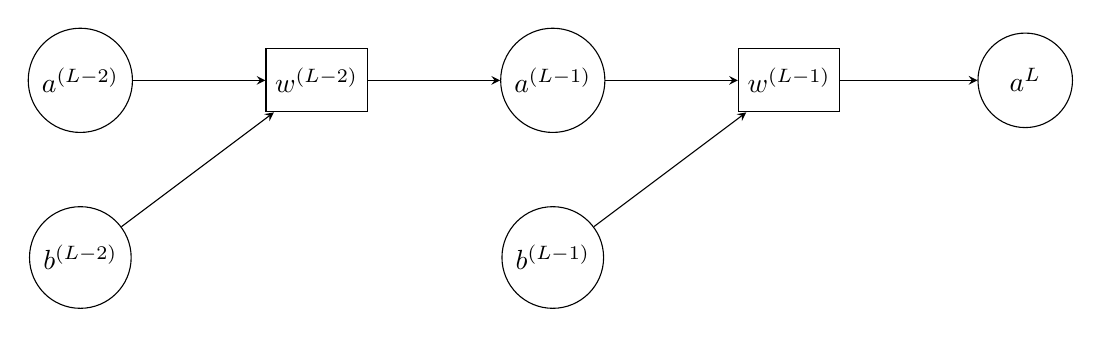
\begin{tikzpicture}[x=1.5cm, y=1.5cm,  >=stealth]
        \tikzstyle{unit}=[draw,shape=circle,minimum size=1.2cm]
        \tikzstyle{weight} =[draw, shape=rectangle, minimum size=.8cm]

        \node[unit](I) at (0, 2){$a^{(L-2)}$};
        \node[unit](b1) at (0,0.5){$b^{(L-2)}$};
        \node[weight](w1) at (2,2){$w^{(L-2)}$};
        \node[unit](H) at (4, 2){$a^{(L-1)}$};
        \node[unit](b2) at (4,0.5){$b^{(L-1)}$};
        \node[weight](w2) at (6,2){$w^{(L-1)}$};
        \node[unit](O) at (8, 2){$a^L$};
        
        \draw[->] (I) -- (w1);
        \draw[->] (w1) -- (H);
        \draw[->] (H) -- (w2);
        \draw[->] (w2) -- (O);
        \draw[->] (b1) -- (w1);
        \draw[->] (b2) -- (w2);
        
        \end{tikzpicture}
	\caption[]{Einfaches Neural Network mit nur einem Neuron pro Layer}
    \label{fig:simpleNetwork}
    Quelle: Eigene Darstellung, 2020
\end{figure}


\begin{figure}[t]
    \centering
    \begin{tikzpicture}[x=1.5cm, y=1.5cm,  >=stealth]
        \tikzstyle{unit}=[draw,shape=circle,minimum size=1.2cm]
        \tikzstyle{weight} =[draw, shape=rectangle, minimum size=.8cm]

        \node[weight](w) at (0, 2){$w^{(L-1)}$};
        \node[weight](a) at (0, 1){$a^{(L-1)}$};
        \node[weight](b) at (0,0){$b^{(L-1)}$};
        \node[weight](z) at (2, 1){$z^{(L)}$};
        \node[weight](aL) at (4,1){$a^{(L)}$};
        \node[unit](c) at (6,1){$C$};
        \node[weight](y) at (6,0){$y$};

        \draw[->] (w) -- (z);
        \draw[->] (a) -- (z);
        \draw[->] (b) -- (z);
        \draw[->] (z) -- (aL);
        %\path [line] (aL) -- node [text width=2.5cm,midway,above ]{$\hat{y}$} (c);
        \draw[->] (aL) -> node [text width=2.5cm,midway,above,align=center ] {$\hat{y}$} (c);

        \draw[->] (y) -- (c);

        \end{tikzpicture}
    \caption[]{Explizite Darstellung Einflüsse der Verlustfunktion des Output Layers}
    \label{fig:unfoldedCost}
    Quelle: Eigene Darstellung, 2020
\end{figure}

Stellt man sich ein möglichst einfaches \ac{NN} mit Hidden Layer vor, erhält man das in Abbildung \ref{fig:simpleNetwork} dargestellte \ac{NN}. Dieses enthält pro Layer nur ein Neuron sowie einen Bias. Alle Gewichte eines Layers wurden für eine bessere Übersichtlichkeit als ein Element repräsentiert. Das heißt, $w^{(L-n)}$ stellt jeweils einen Vektor mit zwei Elementen dar. $a^{L}$ bzw. $a^{(L-n)}$ bezeichnen die Aktivierung - also die finale Ausgabe - des Neurons.

\begin{equation} \label{eq:formulaZ}
    z^{(L)} = w^{(L-1)} a^{(L-1)} + b^{(L-1)}
\end{equation}

In Abbildung \ref{fig:unfoldedCost} sind die Einflüsse auf die Verlustfunktion für den Output Layer $C$ dargestellt. Es ist zu erkennen, dass die Eingänge in die gewichtete Summe $z^{(L)}$ des Output Layers sich aus den Gewichten $w^{(L-1)}$, der Aktivierung des letzten Hidden Layers $a^{(L-1)}$ und dem Bias $b^{(L-1)}$ zusammensetzten. Die entsprechende Formel ist in Gleichung \ref{eq:formulaZ} dargestellt. Das Ergebnis von $z^{(L)}$ wird anschließend in die Aktivierungsfunktion $\sigma$ gegeben, wodurch die Aktivierung des Output Layers $a^{(L)}$ berechnet wird. Diese stellt auch die Ausgabe des \ac{NN} dar, welche als \textit{\^{y}} bezeichnet wird. Mit der Ausgabe des \ac{NN} und dem tatsächlich erwarteten Wert - $y$ - wird anschließend die Verlustfunktion berechnet. Soll also der Fehler des \ac{NN} verkleinert werden, müssen die drei Eingangswerte $w^{(L-1)}$, $a^{(L-1)}$ und $b^{(L-1)}$ angepasst werden. 

%$a^{(L-1)}$ stellt hierbei einen Sonderfall da. Da dies die Aktivierung des vorherigen Layers ist, hängt diese wiederum von den drei selben Eingangssignalen - nur einen Layer vorher, also hier $w^{(L-2)}$, $a^{(L-2)}$ und $b^{(L-2)}$ - ab. Daher soll zunächst die Anpassung von $w^{(L-1)}$ und $b^{(L-1)}$ betrachtet werden.

Wie in Gleichung \ref{eq:defDeltaEdef} dargestellt, muss der Fehler des \ac{NN} mittels partieller Ableitung auf jeden Einflussfaktor zurückgeführt werden. Hierbei wird die Kettenregel angewendet, die einzelnen Glieder kann man aus Abbildung \ref{fig:unfoldedCost} ablesen. Hierfür beginnt man bei dem Element dessen Anpassung vorgenommen werden soll und wandert den Graph weiter, bis man bei $C$ angekommen ist. Die einzelnen Terme der Kettenregel bestehen dann aus der partiellen Ableitung des nächsten Elements im Pfad über das aktuelle Element. Geht man so - beginnend mit dem Element mit $w^{(L-1)}$ - vor, erhält man Gleichung \ref{eq:chainrule_simple_network}.

\begin{equation} \label{eq:chainrule_simple_network}
    \frac{\partial C }{\partial w^{(L-1)}} =  
    \frac{\partial z^{(L)} }{\partial w^{(L-1)}}
    \frac{\partial a^{(L)} }{\partial z^{(L)}}
    \frac{\partial C }{\partial a^{(L)}}
\end{equation}

Berechnet man die entsprechenden Ableitungen, erhält man Gleichung \ref{eq:ableitung_chainrule_simple}.
\begin{equation} \label{eq:ableitung_chainrule_simple}
    \frac{\partial C }{\partial w^{(L-1)}} = 
    a^{(L-1)} \sigma'(z^{(L)})
    2(a^{(L)}-y)
\end{equation}

Der vorderste Teil der rechten Seite der Gleichung ist die partielle Ableitung von der gewichteten Summe $z^{(L)}$ über das Gewicht $w^{(L-1)}$. Der mittlere Teil der Gleichung stellt die Ableitung der gewählten Aktivierungsfunktion $\sigma$ dar und der hinterste Teil ist die Ableitung der gewählten Verlustfunktion. In Gleichung \ref{eq:ableitung_chainrule_simple} wurde hierfür Gleichung \ref{eq:mse} verwendet.

Für die Berechnung des Bias $b^{(L-1)}$ kann der Pfad von $C$ bis $z^{(L)}$ übernommen werden. Es ändert sich also nur etwas im vordersten Glied der Gleichungen \ref{eq:chainrule_simple_network} und \ref{eq:ableitung_chainrule_simple}. Außerdem ist der Bias eine Konstante, seine Ableitung ($1$)  wird nicht dargestellt.

\begin{equation}
    \frac{\partial C }{\partial b^{(L-1)}} =  
    \frac{\partial z^{(L)} }{\partial b^{(L-1)}}
    \frac{\partial a^{(L)} }{\partial z^{(L)}}
    \frac{\partial C }{\partial a^{(L)}} =  \sigma'(z^{(L)})
    2(a^{(L)}-y)
\end{equation}

Die Ergebnisse für $\frac{\partial C }{\partial w^{(L-1)}}$  bzw. $\frac{\partial C }{\partial w^{(L-1)}}$ können in Gleichung \ref{eq:updateW} bzw. \ref{eq:updateB} eingesetzt werden, um das neue Gewicht und den neuen Bias bestimmen zu können. Die Aktivierung des Neuron im vorherigen Layer - $a^{(L-1)}$ - lässt sich nicht direkt anpassen. Sie hängt vom Gewicht, Bias und Aktivierung der vorherigen Schicht ab. Also muss hier der Fehler mit den selben Gleichungen berechnet werden. Hierfür wird zunächst der Einfluss von $a^{(L-1)}$ auf den Fehler $C$ benötigt, da dieser der Fehler ist, der auf die vorherige Schicht verteilt wird. Auch hier ändert sich nur der vorderste Teil des Pfades, sowie dementsprechend das Ergebnis der Ableitung.

\begin{equation} \label{eq:partialCpartialaL-1}
    \frac{\partial C }{\partial a^{(L-1)}} =  
    \frac{\partial z^{(L)} }{\partial a^{(L-1)}}
    \frac{\partial a^{(L)} }{\partial z^{(L)}}
    \frac{\partial C }{\partial a^{(L)}} = w^{(L-1)}\sigma'(z^{(L)})
    2(a^{(L)}-y)
\end{equation}

Nachdem nun alle Einflüsse auf den Output Layer berechnet sind, kann ein Schritt weiter zurück gegangen werden. Im \ac{NN} aus Abbildung \ref{fig:simpleNetwork} ist dies der Input Layer $L-2$. Die explizite Darstellung aller Einflüsse inklusive diesem Layer ist in Abbildung \ref{fig:unfoldedCost2} dargestellt. Wie zu sehen ist, wurden nur die zwei Spalten ganz links zum Diagramm aus Abbildung \ref{fig:unfoldedCost} hinzugefügt. Dank der Kettenregel, spiegelt sich dies auch in den Gleichungen für die neuen Elemente $w^{(L-2)}$, $a^{(L-2)}$, $b^{(L-2)}$ und $z^{(L-1)}$ wieder. In Gleichung \ref{eq:calcWL-2} ist die Berechnung für den Einfluss des Gewichts $w^{(L-2)}$ dargestellt.

\begin{equation} \label{eq:calcWL-2}
    \frac{\partial C }{\partial w^{(L-2)}} = 
    \frac{\partial z^{(L-1)} }{\partial w^{(L-2)}}
    \frac{\partial a^{(L-1)} }{\partial z^{(L-1)}}
    \frac{\partial C }{\partial a^{(L-1)}} = 
    a^{(L-2)}\sigma'(z^{(L-1)}) \frac{\partial C}{\partial a^{(L-1)}}
\end{equation}

Der letzte Term des mittleren bzw. letzten Teils der Gleichung stellt dabei das Ergebnis aus Gleichung \ref{eq:partialCpartialaL-1} dar. Wie zu erkennen ist, erhält man das Ergebnis des aktuellen Layers also dadurch, dass man die Berechnung für den nachfolgendem Layer um weitere Terme ergänzt. Dieses zurückführen des Fehlers ist der Grund, weshalb diese Methode Backpropagation genannt wird. Hätte das \ac{NN} noch weitere Schichten, würde dieser Schritt des Erweiterns der Formel immer wiederholt. Da die Terme der Kettenregel separat berechnet werden können, muss also immer nur der neue Teil berechnet werden, wodurch der Algorithmus effizient durchgeführt werden kann.\todo{Quelle für effizienz}

\begin{figure}[t]
    \centering
    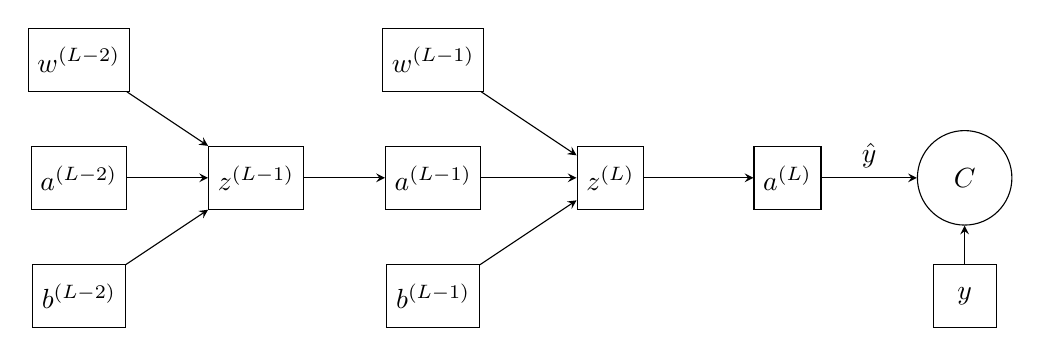
\begin{tikzpicture}[x=1.5cm, y=1.5cm,  >=stealth]
        \tikzstyle{unit}=[draw,shape=circle,minimum size=1.2cm]
        \tikzstyle{weight} =[draw, shape=rectangle, minimum size=.8cm]

        \node[weight](w-2) at (0, 2){$w^{(L-2)}$};
        \node[weight](a-2) at (0, 1){$a^{(L-2)}$};
        \node[weight](b-2) at (0,0){$b^{(L-2)}$};
        \node[weight](z-2) at (1.5, 1){$z^{(L-1)}$};
        \node[weight](w-1) at (3, 2){$w^{(L-1)}$};
        \node[weight](a-1) at (3, 1){$a^{(L-1)}$};
        \node[weight](b-1) at (3,0){$b^{(L-1)}$};
        \node[weight](z-1) at (4.5, 1){$z^{(L)}$};
        \node[weight](aL) at (6,1){$a^{(L)}$};
        \node[unit](c) at (7.5,1){$C$};
        \node[weight](y) at (7.5,0){$y$};

        \draw[->] (w-2) -- (z-2);
        \draw[->] (a-2) -- (z-2);
        \draw[->] (b-2) -- (z-2);
        \draw[->] (z-2) -- (a-1);
        \draw[->] (w-1) -- (z-1);
        \draw[->] (a-1) -- (z-1);
        \draw[->] (b-1) -- (z-1);
        \draw[->] (z-1) -- (aL);
        %\path [line] (aL) -- node [text width=2.5cm,midway,above ]{$\hat{y}$} (c);
        \draw[->] (aL) -> node [text width=2.5cm,midway,above,align=center ] {$\hat{y}$} (c);

        \draw[->] (y) -- (c);

        \end{tikzpicture}
    \caption[]{Explizite Darstellung Einflüsse der Verlustfunktion des gesamten Neural Networks}
    \label{fig:unfoldedCost2}
    Quelle: Eigene Darstellung, 2020
\end{figure}

Typischerweise haben \ac{NN} mehr als ein Neuron pro Layer, daher müssen die oben genannten Formeln noch leicht angepasst werden. In Gleichungen \ref{eq:forwardMulti} sind die Formeln für das Vorwärtsdurchlaufen des \ac{NN} dargestellt. Da nun mehrere Neuronen im Output Layer vorhanden sind - $N_L$ - muss über diese summiert werden. Anschließend muss für den quadratischen Mittelwert noch durch die Anzahl der Neuronen geteilt werden (siehe Formel 1 in Abbildung \ref{eq:forwardMulti}).

Auch die gewichtet Summe in jedem Neuron hängt nun von allen Aktivierungen des vorherigen Layer ($N_{(L-1)}$) ab, so dass hier ebenfalls über diese summiert werden muss. Da es nun mehrere Neuronen pro Layer - und somit mehrere gewichtete Summen pro Layer - gibt, wird mittels dem Index  $j$ noch spezifiziert, welches Neuronen gerade berechnet wird.

\begin{equation} \label{eq:forwardMulti}
    \begin{split}
        &C=\frac{1}{N_{L}} \sum_{j=1}^{N_{L}}\left(a_{j}^{(L)}-y_{j}\right)^{2} \\
        &z_{j}^{(L)}=\sum_{k=1}^{N_{L-1}} w_{j k}^{(L-1)} a_{k}^{(L-1)}+b_{j}^{(L-1)} \\
        &a_{j}^{(L)}=\sigma\left(z_{j}^{(L)}\right)
    \end{split}
\end{equation}


Wendet man die gleiche Vorgehensweise und Überlegung wie für das des einfachen \ac{NN} an und nutzt zusätzlich die neue Notation, erhält man für den Einfluss das Gewichtes $w_{j k}^{(L-1)}$ Gleichung \ref{eq:infWLayer1}. Ähnlich wie beim einfachen \ac{NN} unterscheidet sich die Formel für ein Bias nur durch die geänderten Formelzeichen, daher wird auf eine explizite Darstellung verzichtet.


\begin{equation} \label{eq:infWLayer1}
    \frac{\partial C}{\partial w_{j k}^{(L-1)}}=\frac{\partial z_{j}^{(L)}}{\partial w_{j k}^{(L-1)}} \frac{\partial a_{j}^{(L)}}{\partial z_{j}^{(L)}} \frac{\partial C}{\partial a_{j}^{(L)}}
\end{equation}

Größere Änderungen gibt es für den Einfluss der Aktivierung $a_{k}^{(L-1)}$. Da jedes Neuron in diesem Hidden Layer mit jedem Neuron im Output Layer verbunden ist, hat es auch Einfluss auf den Fehler jedes Neurons im Output Layer. Möchte man also den gesamten Fehler eines Neurons im Hidden Layer berechnen, muss man die Summe über alle zurückgeführten Fehler aus dem Output Layer bilden (siehe Gleichungen \ref{eq:infALayer1}).

\begin{equation} \label{eq:infALayer1}
        \frac{\partial C}{\partial a_{k}^{(L-1)}}=\sum_{j=1}^{N_{L}} \frac{\partial z_{j}^{(L)}}{\partial a_{k}^{(L-1)}} \frac{\partial a_{j}^{(L)}}{\partial z_{j}^{(L)}} \frac{\partial C}{\partial a_{j}^{(L)}} \\
\end{equation}

Neben dem Hinzufügen der neuen Notation mit Indizes und der Summe (Ich gehe mal davon aus das hier klar ist welche Summe gemeint ist), gibt es keine Änderungen zum Fall im einfachen \ac{NN}. Dies lässt sich auch beobachten, wenn ein weiterer Schritt zurück gegangen wird. Also Elemente im Layer $L-2$ betrachtet werden. Für das Gewicht $w_{j k}^{(L-2)}$ wird die Formel in Gleichung \ref{eq:infWL-2} dargestellt. Genau wie beim einfachen \ac{NN}, wurde das Ergebnis des vorherigen Layers um zwei weitere Terme ergänzt. Ähnlich sieht es bei der Aktivierung aus, hier enthält der letzte Term in Summenzeichen aus Gleichung \ref{eq:infALayer1} immer den Weg vom aktuellen Layer bis zu $C$, so dass die zwei anderen Terme in der Summe nur auf den aktuellen Layer angepasst werden müssen. 

\begin{equation} \label{eq:infWL-2}
    \frac{\partial C}{\partial w_{j k}^{(L-2)}}=\frac{\partial z_{j k}^{(L-1)}}{\partial w_{j k}^{(L-2)}} \frac{\partial a_{j}^{(L-1)}}{\partial z_{j}^{(L-1)}} \frac{\partial C}{\partial a_{j}^{(L-1)}}
\end{equation}

Verwendet man die hergeleiteten Gleichungen und erweitert sie gegebenenfalls für weitere Hidden Layer, ist man in der Lage die Anpassungen aller Gewichte und Bias in einem \ac{NN} zu berechnen. Der komplette Lernprozess besteht dann aus den folgenden vier Schritten:

\begin{enumerate}
    \item Durchführen eines Vorwärtsdurchlaufs um die Ausgabe des Output Layers zu erhalten (\textit{\^{y}})
    \item Ausrechnen der Verlustfunktion ($C(w,b)$), um den Fehler des \ac{NN} zu erhalten
    \item Berechnen der Gradienten von $C(w,b)$ im Bezug auf alle Gewichte und Bias im \ac{NN}
    \item Anpassen der Gewichte und Bias im Netzwerk anhand der berechneten Gradienten und den Ausgangswerten
\end{enumerate}